This is the description of the methods. 

\section{Which aspect types do I use?}
One inherent drawback of computational methods is exactly their one unifying characteristic: their computability. Sadly, the requirement for computability means, in many cases, sacrificing the nuance that comes with more qualitative approaches. In this concrete case this means settling for a single aspect classification system. A consequence of the glut of literature in the field is a glut of classification systems to go with it, each with their own idiosyncrasies and each having their own advantages and drawbacks. I will attempt to discuss what I see as the main candidates before deciding on one system and explaining this decision - NO - this was done in aspectology already!!!!SEE ABOVE

reason is of course the contribution to the linguistic community: computational approaches to language have SPURRED ON LOTS OF PROGRESS (cf Chomsky!!!). 

The framework I decided on was Uniform Meanign Representation (UMR) \citep{umr}.

\subsection{UMR}
UMR \citep{umr} was introduced in order to expand and further generalise the attempt to design an abstract semantic representation, as was most successfully pioneered by \citet{amr} with Abstract Meaning Representation (AMR). In contrast to AMR, UMR aims to be a typologically-informed abstraction away from English structures, making it more suitable for other similar languages, or, in their own words, making it "a practical and cross-linguistically valid meaning representation designed to meet the needs of a wide range of NLP applications" \citep{umr}.


\subsection*{Aspect in UMR}
UMR describes the following 5 corse-grained aspect classes: (descriptions taken from \citet{umr}), also depicted in figure \ref{fig:umr_aspect_tree}:
\begin{itemize}
    \item \textbf{state} - an unspecified type of state
    \item \textbf{habitual} - an event that occurs regularly in the past or
    present, including generic statements
    \item \textbf{activity} - an event that has not necessarily ended and may
    be ongoing at Document Creation Time (DCT)
    \item \textbf{endeavour} - a process that ends without reaching completion
    (i.e., termination)
    \item \textbf{performance} - a process that reaches a completed result
    state
\end{itemize}

\begin{figure}
    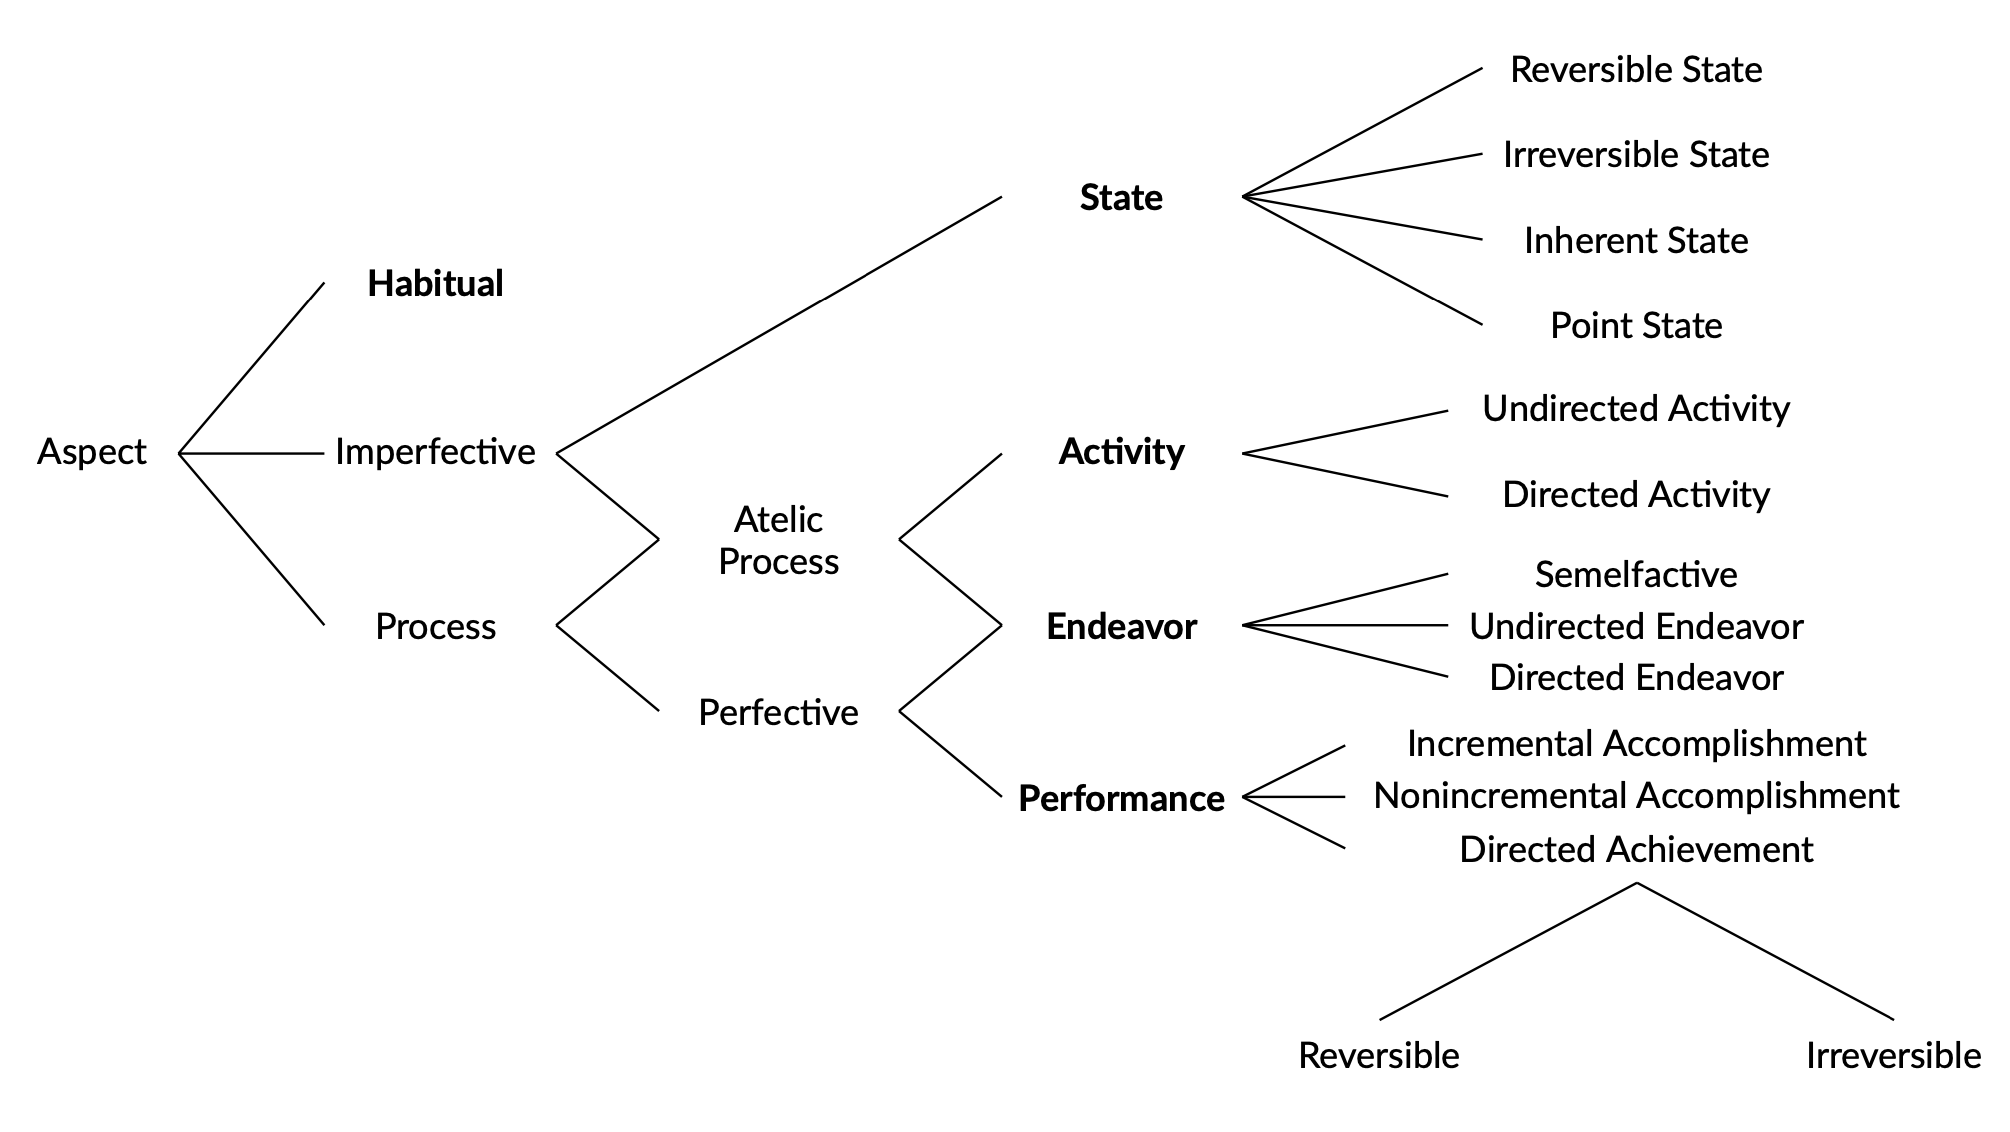
\includegraphics[width=\textwidth]{img/umr_aspct_tree.png}
    \caption{UMR aspect classification tree \citep{umrslides2022}}
    \label{fig:umr_aspect_tree}
\end{figure}

How these relate to other aspectual classes can be shown in table \ref{table:aspect_classes_comparison}.

Interesting to note is that these classes conflate the distinction made earlier between lexical and grammatical aspect, most clearly in the class "habitual", which is a paradigmatic example of an outer aspect, rather than one inherent in the verb event itself. However, as can be seen in figure \ref{fig:umr_aspect_tree}, while classes which would usually be seen as grammatical aspect are to be found nearer the top of the tree (on the left), the leaves further down the tree are more examples of \emph{Aktionsarten}. That \citet{umr} make no mention of these different types of aspect is not necessarily surprising, given one of the main design goals of UMR being scalability, itself entailing learnability for annotators. As we have seen (HAVE WE?), the theoretical distinction of inner and outer aspect is "very difficult to apply in practice" \citep{Dahl1985TenseAA}, hence a clear separation would often be difficult - and indeed not very fruitful - for annotators. This conflation of two phenomena, however, can also be an advantage, since it shows the relationship between classes of each type (i.e. that \emph{irreversible states} are imperfective and \emph{directed achievements} perfective etc.), subsuming them all into \emph{one} semantic parameter space concerning aspect. A further advantage of UMR is the flexibility of annotation levels that can be seen in figure \ref{fig:umr_aspect_tree}. This allows for annotation both at a fine-grained level (using the classes at the bottom of the tree), but also on a more coarse-grained level if instances are unclear or annotators unsure.

\begin{table}[]
    \begin{adjustbox}{width=\textwidth}
    \begin{tabular}{|l|l|l|l|l|l|l|}
    \hline
    \citet*{vendler57} &  \citet*{moens-steedman-1988-temporal}& \citet*{egg2005flexible} & \multicolumn{3}{l}{\citet*{annotAndAutoClassOfAspectCat}}  \vline & \citet{umr} \\ \hline \hline
\multirow{2}{*}{state}         & state                      & stative predicate     & \multicolumn{3}{l}{stative} \vline & \textbf{state} \\ \cline{2-7}
                               & (habitual state)           & (CHECK THIS)          & \multicolumn{3}{l}{-} \vline & \textbf{habitual} \\ \hline
activity                       & \multirow{2}{*}{process}   & process predicate     & \multirow{5}{*}{dynamic} & \multicolumn{2}{l}{unbounded} \vline & \textbf{activity} \\ \cline{1-1}\cline{3-3}\cline{5-7}
\multirow{2}{*}{accomplishment}&                            & intergressive predicate&      & \multirow{4}{*}{bounded} &  extended/no change & \textbf{endeavour} \\ \cline{2-3}\cline{6-7}
                               & culminated process         & change predicate      &       &  & extended/change & \textbf{performance}\\ \cline{1-3}\cline{6-7}
\multirow{2}{*}{achievement}   & point                      & intergressive predicate&      &  & punctual/no change & \textbf{endeavour} \\ \cline{2-3} \cline{6-7}
                               & culmination                & change predicate      &       &  & punctual/change & \textbf{performance} \\ \hline

    \end{tabular}
    \end{adjustbox}
    \caption{Comparison of aspectual classes. Adapted and extended from \citet*{annotAndAutoClassOfAspectCat}.}
    \label{table:aspect_classes_comparison}
\end{table}


\section{Use of approximative LMs as sources of linguistic knowledge??}
\section{Where do LLMs fail?}


